\documentclass[a4paper,11pt]{article}
\title{Faraday's Law PAG}
\author{Izaak van Dongen}

% make the document take up more of the page
\usepackage[margin=1in,headheight=13.6pt]{geometry}

% so the title can be accessed by fancyhdr (and is automatically correctly
% spelled etc)
\makeatletter
\let\thetitle\@title
\makeatother

% custom document header/footer
\usepackage{fancyhdr}
\usepackage{lastpage}

\pagestyle{fancy}
\fancyhf{}
\lhead{\thetitle}
\rhead{Izaak van Dongen}
\rfoot{Page \thepage\ of \pageref{LastPage}}

%% fonts
%\usepackage[p,osf]{cochineal}
%\usepackage[scale=.95,type1]{cabin}
%\usepackage[cochineal,bigdelims,cmintegrals,vvarbb]{newtxmath}
%% fixed width font with 80 chars per listing line
%\usepackage[scaled=.94]{newtxtt}
%\usepackage[cal=boondoxo]{mathalfa}
\usepackage{amsfonts}

% provides eg uptau
\usepackage{upgreek}

% maths symbols and other stuff (supersedes the ams* packages)
\usepackage{mathtools}

% for typesetting differentials
\usepackage{commath}

%
\usepackage{yfonts}
\def\initdefault{yinit} % fix weird font thing

% define starting paragraph letter stuff
\usepackage{lettrine}
\setcounter{DefaultLines}{4}
\setlength{\DefaultFindent}{0.5em}
\setlength{\DefaultNindent}{0em}
\renewcommand{\LettrineFontHook}{\usefont{U}{yinit}{m}{n}}


% no paragraph indent
\usepackage[parfill]{parskip}

% pretty table rules and multirow entries. Also page-breaking tables
\usepackage{booktabs}
\usepackage{multirow}
\usepackage{longtable}

% plotting mathematical functions (needs version request)
\usepackage{pgfplots}
\pgfplotsset{compat=1.15}

% \url function and clickable table of contents. no ugly red boxes though
\usepackage[hidelinks]{hyperref}

% For framing definitions
\usepackage[framemethod=tikz]{mdframed}
\usepackage[most]{tcolorbox}

\newtcolorbox{definition}{
freelance,
before=\par\vspace{2\bigskipamount}\noindent,
after=\par\bigskip,
frame code={
  \node[
  anchor=south west,
  inner xsep=8pt,
  xshift=8pt,
  rounded corners=5pt,
  font=\bfseries\color{white},
  fill=gray] at (frame.north west) (tit) {\strut Definition:};
  \draw[
  line width=3pt,
  rounded corners=5pt,gray
  ] (tit.west) -| (frame.south west) -- ([xshift=15pt]frame.south west);
},
interior code={},
top=2pt
}

% for better table of contents stuff, providing the \listof* commands and not
% listing the tables in the table of contents
\usepackage[nottoc,notlof,notlot]{tocbibind}

% more advanced handling of utf8 and fonts or something. apparently good to have
\usepackage[utf8]{inputenc}
\usepackage[T1]{fontenc}

% somehow this fixes ~ signs in listing environments
\usepackage{lmodern}

% bibliography management with square braces for citations
\usepackage[square,numbers]{natbib}

% graphics, like eps files and stuff (supersedes graphics)
\usepackage{graphicx}

% used to horizontally align floats
\usepackage{subcaption}

% used for figures
\usepackage{float}

% needed for colouring and stuff (xcolor supersedes color)
\usepackage{xcolor}

\definecolor{codegreen}{rgb}{ 0,0.6,0}

% listings of code
\usepackage{minted}
\setminted{breaklines,
           breakbytokenanywhere,
           linenos
}
\usemintedstyle{friendly}
% bigger line numbers
\renewcommand\theFancyVerbLine{\footnotesize\arabic{FancyVerbLine}}

% that can break across pages while being captioned figures
\usepackage{caption}
\newenvironment{longlisting}
{\addvspace{\baselineskip}\captionsetup{type=listing}}
{\addvspace{\baselineskip}}

% allow maths to break across pages
\allowdisplaybreaks

\usepackage[separate-uncertainty]{siunitx}

\begin{document}
    \maketitle%\thispagestyle{empty} % no page number under title

\begin{longlisting}
\inputminted{R}{analyse.r}
\end{longlisting}

There seems to be a roughly linear relationship between max induced EMF and
velocity (fig \ref{fig_peak}). This would make sense as Faraday's law states
that EMF is proportional to rate of change of flux, which when the field is
uniform is in turn proportional to velocity. However the data sample is probably
much too closely spaces to make any conclusions, as any roughly analytic
function of displacement would probably produce a similar plot.

\begin{figure}[b]
\centering
\begin{subfigure}{.5\textwidth}
    \centering
    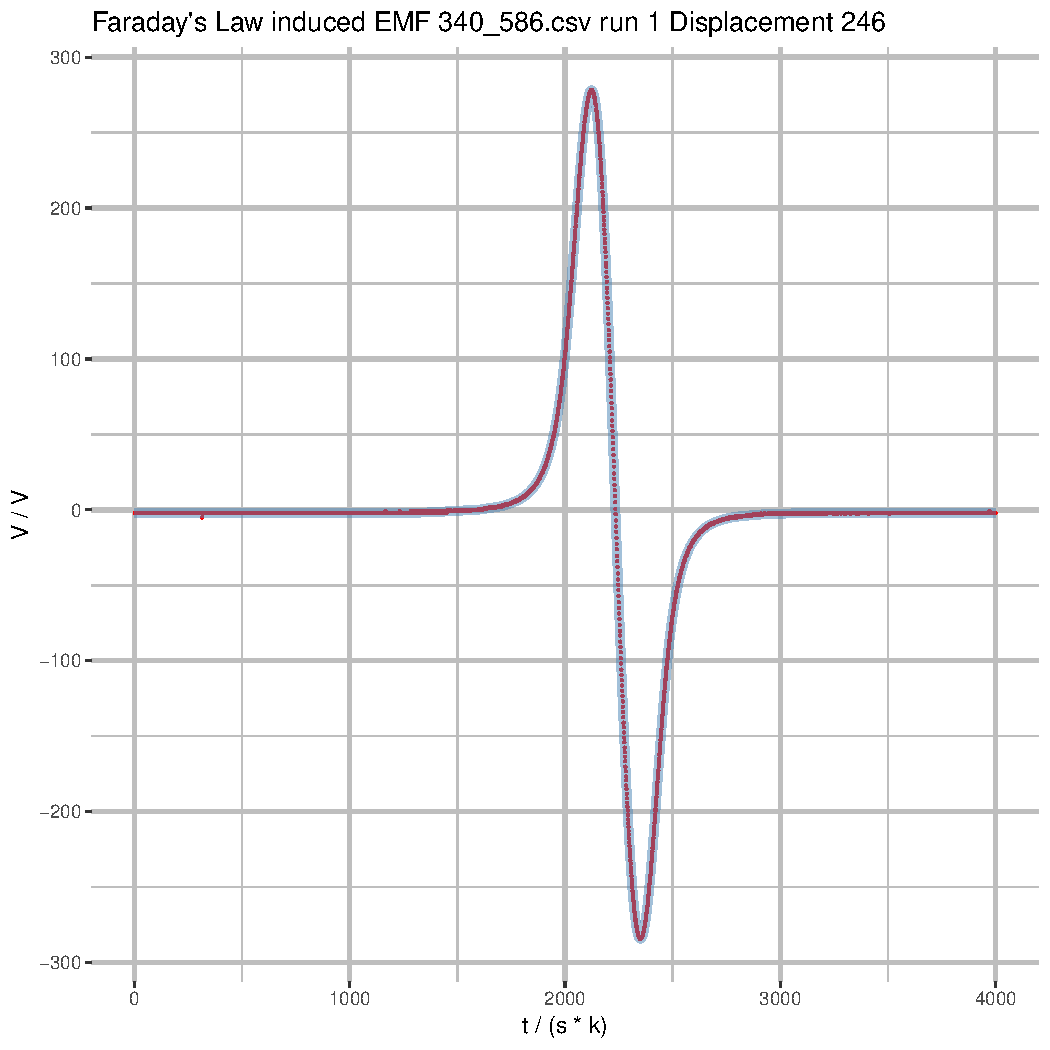
\includegraphics[width=\textwidth,page=1]{Rplots.pdf}
\end{subfigure}%
\begin{subfigure}{.5\textwidth}
    \centering
    \includegraphics[width=\textwidth,page=2]{Rplots.pdf}
\end{subfigure}
\begin{subfigure}{.7\textwidth}
    \centering
    \includegraphics[width=\textwidth,page=3]{Rplots.pdf}
\end{subfigure}
\caption{\(d = \SI{246}{\milli\metre}\)}
\end{figure}

\begin{figure}[b]
\centering
\begin{subfigure}{.5\textwidth}
    \centering
    \includegraphics[width=\textwidth,page=4]{Rplots.pdf}
\end{subfigure}%
\begin{subfigure}{.5\textwidth}
    \centering
    \includegraphics[width=\textwidth,page=5]{Rplots.pdf}
\end{subfigure}
\begin{subfigure}{.7\textwidth}
    \centering
    \includegraphics[width=\textwidth,page=6]{Rplots.pdf}
\end{subfigure}
\caption{\(d = \SI{100}{\milli\metre}\)}
\end{figure}

\begin{figure}[b]
\centering
\begin{subfigure}{.5\textwidth}
    \centering
    \includegraphics[width=\textwidth,page=7]{Rplots.pdf}
\end{subfigure}%
\begin{subfigure}{.5\textwidth}
    \centering
    \includegraphics[width=\textwidth,page=8]{Rplots.pdf}
\end{subfigure}
\begin{subfigure}{.7\textwidth}
    \centering
    \includegraphics[width=\textwidth,page=9]{Rplots.pdf}
\end{subfigure}
\caption{\(d = \SI{140}{\milli\metre}\)}
\end{figure}

\begin{figure}[b]
\centering
\begin{subfigure}{.5\textwidth}
    \centering
    \includegraphics[width=\textwidth,page=10]{Rplots.pdf}
\end{subfigure}%
\begin{subfigure}{.5\textwidth}
    \centering
    \includegraphics[width=\textwidth,page=11]{Rplots.pdf}
\end{subfigure}
\begin{subfigure}{.7\textwidth}
    \centering
    \includegraphics[width=\textwidth,page=12]{Rplots.pdf}
\end{subfigure}
\caption{\(d = \SI{160}{\milli\metre}\)}
\end{figure}

\begin{figure}[b]
\centering
\begin{subfigure}{.5\textwidth}
    \centering
    \includegraphics[width=\textwidth,page=13]{Rplots.pdf}
\end{subfigure}%
\begin{subfigure}{.5\textwidth}
    \centering
    \includegraphics[width=\textwidth,page=14]{Rplots.pdf}
\end{subfigure}
\begin{subfigure}{.7\textwidth}
    \centering
    \includegraphics[width=\textwidth,page=15]{Rplots.pdf}
\end{subfigure}
\caption{\(d = \SI{180}{\milli\metre}\)}
\end{figure}

\begin{figure}[b]
\centering
\begin{subfigure}{.5\textwidth}
    \centering
    \includegraphics[width=\textwidth,page=16]{Rplots.pdf}
\end{subfigure}%
\begin{subfigure}{.5\textwidth}
    \centering
    \includegraphics[width=\textwidth,page=17]{Rplots.pdf}
\end{subfigure}
\begin{subfigure}{.7\textwidth}
    \centering
    \includegraphics[width=\textwidth,page=18]{Rplots.pdf}
\end{subfigure}
\caption{\(d = \SI{216}{\milli\metre}\)}
\end{figure}

\begin{figure}[b]
\centering
\begin{subfigure}{.5\textwidth}
    \centering
    \includegraphics[width=\textwidth,page=19]{Rplots.pdf}
\end{subfigure}%
\begin{subfigure}{.5\textwidth}
    \centering
    \includegraphics[width=\textwidth,page=21]{Rplots.pdf}
\end{subfigure}
\begin{subfigure}{.7\textwidth}
    \centering
    \includegraphics[width=\textwidth,page=20]{Rplots.pdf}
\end{subfigure}
\caption{Area plots}
\end{figure}

\begin{figure}[b]
\centering
\begin{subfigure}{.7\textwidth}
    \centering
    \includegraphics[width=\textwidth,page=22]{Rplots.pdf}
\end{subfigure}
\begin{subfigure}{.7\textwidth}
    \centering
    \includegraphics[width=\textwidth,page=23]{Rplots.pdf}
\end{subfigure}
\caption{Peak plots}\label{fig_peak}
\end{figure}

\end{document}
